\section{Numerical methods}\label{sec:FDTD}
This section will give a brief introduction of physical modelling using FDTD methods, including details on stability and quality of the simulations based on these methods.

\subsection{Discretisation}
Using FDTD methods, the continuous 1D wave equation in Eq. \eqref{eq:1dwave} can be discretised into points in space and time. The spatial variable can be discretised using $x_l = lh$ (read: $x$ at location $l$) with integer $l \in [0, \hdots, N]$, distance between two consecutive grid points $h$ (in m), also referred to as the grid spacing, and total number of points $N + 1$ (including the boundaries) where the total number of intervals between the grid points is described as
\begin{equation}\label{eq:numberOfIntervals}
    N = \lfloor L/h\rfloor,
\end{equation}
with $\lfloor \cdot \rfloor$ denoting the flooring operation. The temporal variable can be discretised using $t_n = nk$ with positive integer $n$, time step $k = 1/f_\text{s}$ (in s) and sample rate $f_\text{s}$ (in Hz). The state variable $u$ can then be approximated using $u(x,t) \approx u_l^n$, where grid function $u_l^n$ is the displacement of $u$ at spatial index $l$ and time index $n$. %The total state at time index $n$ is then denoted as vector $\mathbf{u}^n$ with size $N+1$.

The following operators can then be applied to $u_l^n$ to get the following approximations to the derivatives in Eq. \eqref{eq:1dwave}
\begin{subequations}\label{eq:operators}
    \begin{align}
         \delta_{tt}u_l^n &= \frac{1}{k^2}\left(u_l^{n+1}-2u_l^n + u_l^{n-1}\right)\;\;\approx\quad\frac{\partial^2u}{\partial t^2}\label{eq:secondOrderTime}\ ,\\
         \delta_{xx}u_l^n &= \frac{1}{h^2}\left(u_{l+1}^n-2u_l^n + u_{l-1}^n\right)\quad\approx\quad \frac{\partial^2u}{\partial x^2}\ .\label{eq:secondOrderSpace}
    \end{align}
\end{subequations}
Substituting these definitions into Eq. \eqref{eq:1dwave} yields the following finite-difference scheme (FDS)
\begin{equation}\label{eq:FDS}
    \delta_{tt}u_l^n = c^2 \delta_{xx}u_l^n.
\end{equation}
Expanding the operators as in %the Eqs. in
\eqref{eq:operators} and solving for $u_l^{n+1}$ (which is the only unknown) yields the following update equation
\begin{equation}\label{eq:updateEq}
    u_l^{n+1} = 2u_l^n-u_l^{n-1} + \lambda^2 \left(u_{l+1}^n-2u_l^n + u_{l-1}^n\right),
\end{equation}
saying that $u$ at the next time index ($n+1$) can be calculated using only values of $u$ at the current ($n$) and previous time indices ($n-1$). This update can be implemented in software, such as {\tt MATLAB} or {\tt C++}. In Eq. \eqref{eq:updateEq},
\begin{equation}\label{eq:lambdaDef}
    \lambda = \frac{ck}{h}
\end{equation}
is referred to as the Courant number and determines whether the system is stable, as well as the quality and behaviour of the simulation. This will be described in detail in Sections \ref{sec:stability} and \ref{sec:quality}.

In the FDS described in Eq. \eqref{eq:FDS}, the boundary locations are at $l = 0$ and $l = N$. Substituting these locations into Eq. \eqref{eq:updateEq} seemingly shows that grid points outside of the defined domain are needed, namely $u_{-1}^n$ and $u_{N+1}^n$. These can be referred to as \textit{virtual grid points} and can be accounted for %/defined
by using the boundary conditions in Eq. \eqref{eq:continuousBoundaries}. Discretising these yields
\begin{subequations}
    \begin{align}
        u_0^n = u_N^n &= 0 \quad\text{(Dirichlet)}\label{eq:discreteDirichlet}\\
        \delta_{x\cdot} u_0^n = \delta_{x\cdot} u_N^n &= 0 \quad \text{(Neumann)}\label{eq:discreteNeumann}
    \end{align}
\end{subequations}
where 
\begin{equation}
    \delta_{x\cdot}u_l^n = \frac{1}{2h}\left(u_{l+1}^n - u_{l-1}^n\right)\quad \approx\quad \frac{\partial u}{\partial x}
\end{equation}
is a second-order accurate approximation of the first-order spatial derivative. The Dirichlet condition in \eqref{eq:discreteDirichlet} says that the displacement of $u$ at the boundary locations are always 0. In practice, this means that these grid points do not need to be updated and the spatial range of calculation for Eq. \eqref{eq:updateEq} then becomes $l = [1, \hdots, N-1]$. If the Neumann condition is used, the boundary points do need to be updated as these are not necessarily $0$; rather, their `slope' is $0$. Eq. \eqref{eq:discreteNeumann} can then be expanded to yield defnitions for these virtual grid points
\begin{equation}\label{eq:neumannSolution}
    u_{-1}^n = u_1^n \quad \text{and} \quad u_{N+1}^n = u_{N-1}^n\,.
\end{equation}

Now that the full system is described, the output sound can be retrieved by `recording' the state $u_l^n$ in Eq. \eqref{eq:updateEq} at $0 < l < N$ (when using fixed boundary conditions) and listening to that at the given sample rate $f_\text{s}$. Though the output location does not change the behaviour of the system, it will determine the amplitude of different harmonic partials in the system output.

\subsection{Stability}\label{sec:stability}
Discretising continuous equations using numerical methods places limits on the parameters describing it. A wrong choice of parameters could render the system unstable and make it ``explode". In the case of the update in Eq. \eqref{eq:updateEq} it can be shown -- using Von Neumann analysis \cite{Strikwerda1989} -- that the system is stable if
\begin{equation}\label{eq:CFL}
    \lambda \leq 1,
\end{equation}
which is referred to as the Courant-Friedrichs-Lewy (CFL) stability condition. The closer $\lambda$ is to this condition, the higher the quality of the simulation (see Section \ref{sec:quality}) and if $\lambda = 1$, Eq. \eqref{eq:updateEq} provides an exact solution to Eq. \eqref{eq:1dwave} %(this is true for the 1D wave equation)
(see Figures \ref{fig:dispersion}a and \ref{fig:dispersion}b). If $\lambda > 1$ the system will become unstable (see Figure \ref{fig:dispersion}c).
\begin{figure}[t]
    \centering
    % \subfloat[]{\label{fig:lambda1}{ 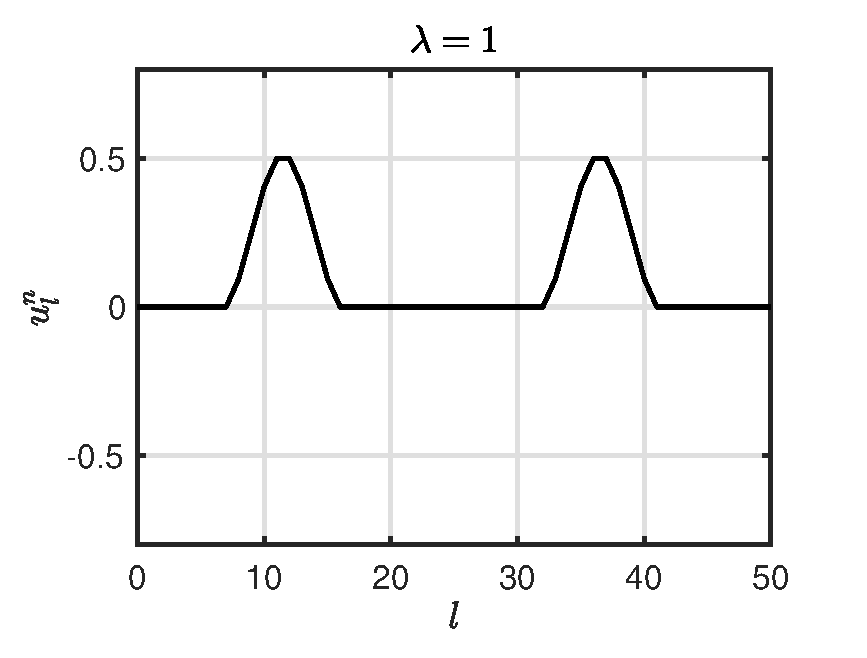
\includegraphics[width=0.3\textwidth]{Figures/ulnLambda1.eps}}}
    % \subfloat[]{\label{fig:lambda0.9}{ 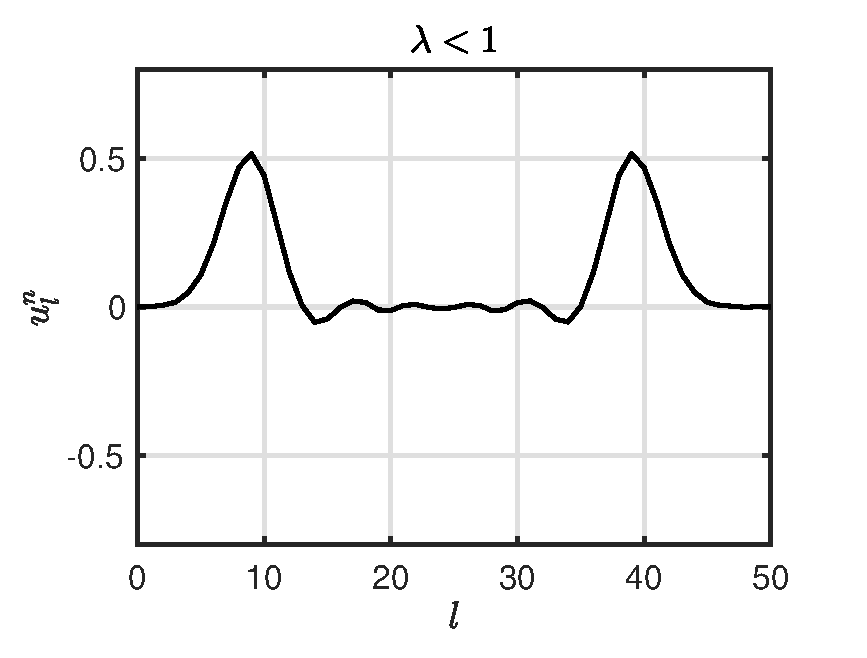
\includegraphics[width=0.3\textwidth]{Figures/ulnLambda09.eps}}}
    % \subfloat[]{\label{fig:lambda1.001}{ 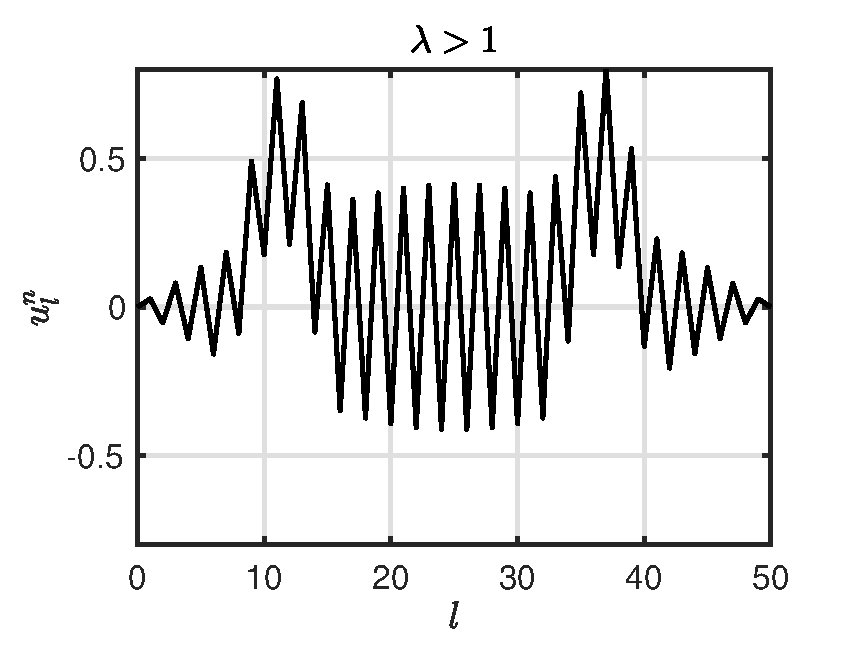
\includegraphics[width=0.3\textwidth]{Figures/ulnLambda1001.eps}}}
    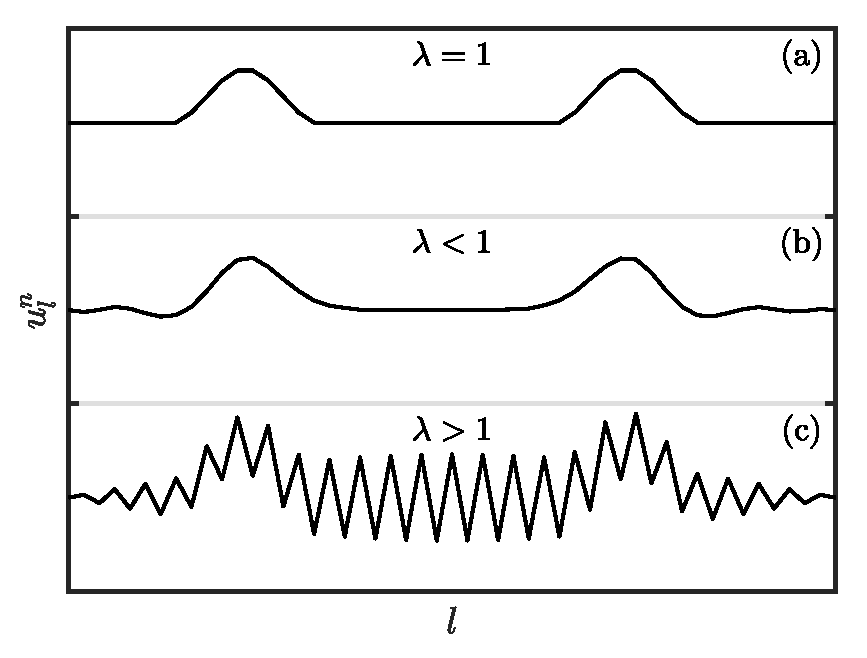
\includegraphics[width=0.8\columnwidth]{Figures/dispersionCompact.eps}
    \caption{State $u_l^n$ with $N = 50$ and $f_\text{s} = 44100$ visualised $\sim\!100$ samples after excitation. (a) If $\lambda = 1$, the solution is exact. (b) If $\lambda < 1$ dispersive behaviour shows. (c) If $\lambda > 1$ the CFL condition in Eq. \eqref{eq:CFL} is not satisfied and the system is unstable.
    \label{fig:dispersion}}
\end{figure}

% discrete boundaries here?
Recalling \eqref{eq:lambdaDef} can rewrite Eq. \eqref{eq:CFL} in terms of grid spacing $h$ to get
\begin{equation}\label{eq:stabilityCond}
    h \geq ck.
\end{equation}
This shows that the CFL condition in \eqref{eq:CFL} puts a lower bound on the grid spacing, determined by the sample rate and wave speed. Usually, the following steps are taken to calculate $\lambda$
\begin{equation}\label{eq:orderOfCalcGrid}
    h := ck,\ \ N := \left\lfloor\frac{L}{h}\right\rfloor, \ \ h := \frac{L}{N}, \ \ \lambda := \frac{ck}{h}.
\end{equation}
In other words, condition \eqref{eq:stabilityCond} is first satisfied with equality and used to calculate integer $N$ according to Eq. \eqref{eq:numberOfIntervals}. Thereafter, $h$ is recalculated based on $N$ and used to calculate $\lambda$. The calculation of $\lambda$ in Eq. \eqref{eq:orderOfCalcGrid} can be compactly rewritten as
\begin{equation}\label{eq:compactLambda}
    \lambda = \frac{ck}{L}\cdot\left\lfloor\frac{L}{ck}\right\rfloor.
\end{equation}
The flooring operation causes the CFL condition in \eqref{eq:CFL} to not always be satisfied with equality and results in a reduced simulation quality described in the following section.

\subsection{Simulation Quality}\label{sec:quality}
As mentioned above, the Courant number $\lambda$ decides the quality of the simulation. Choosing $\lambda < 1$ will decrease this quality in two ways. Firstly, it will decrease the maximum frequency that the simulation is able to produce, i.e., it will decrease the bandwidth of the output sound of the system. See Figure \ref{fig:bandWidths}.

\begin{figure}[t]
    \centering
    % \subfloat[]{\label{fig:bandwidth1}{ 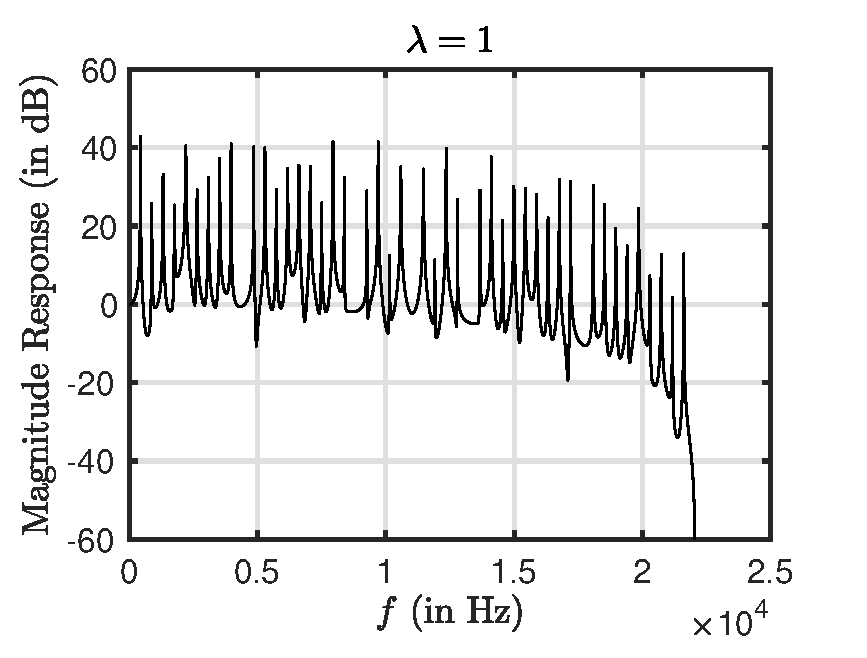
\includegraphics[width=0.3\textwidth]{Figures/bandwidthLambda1.eps}}}
    % \subfloat[]{\label{fig:bandwidth09}{ 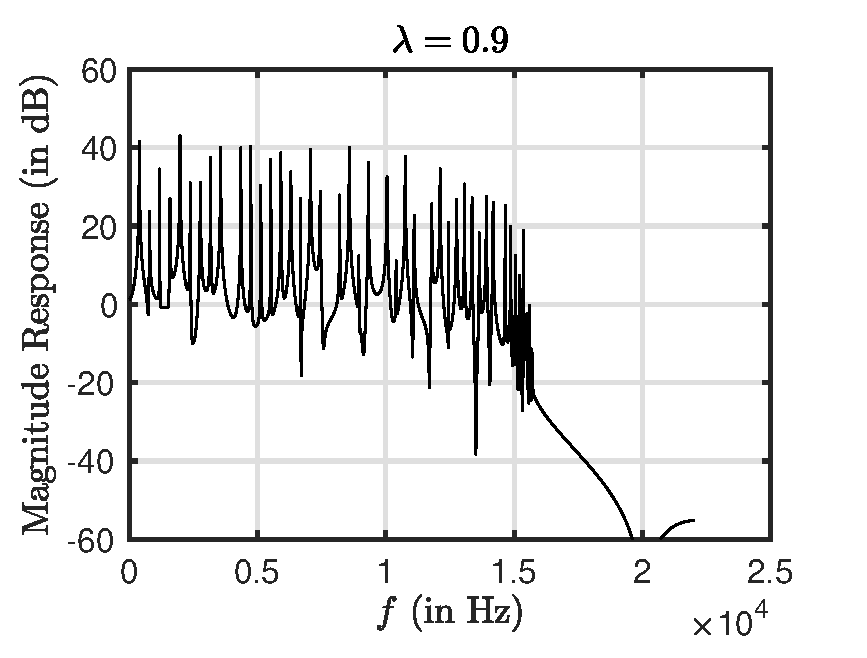
\includegraphics[width=0.3\textwidth]{Figures/bandwidthLambda09.eps}}}
    % \subfloat[]{\label{fig:bandwidth05}{ 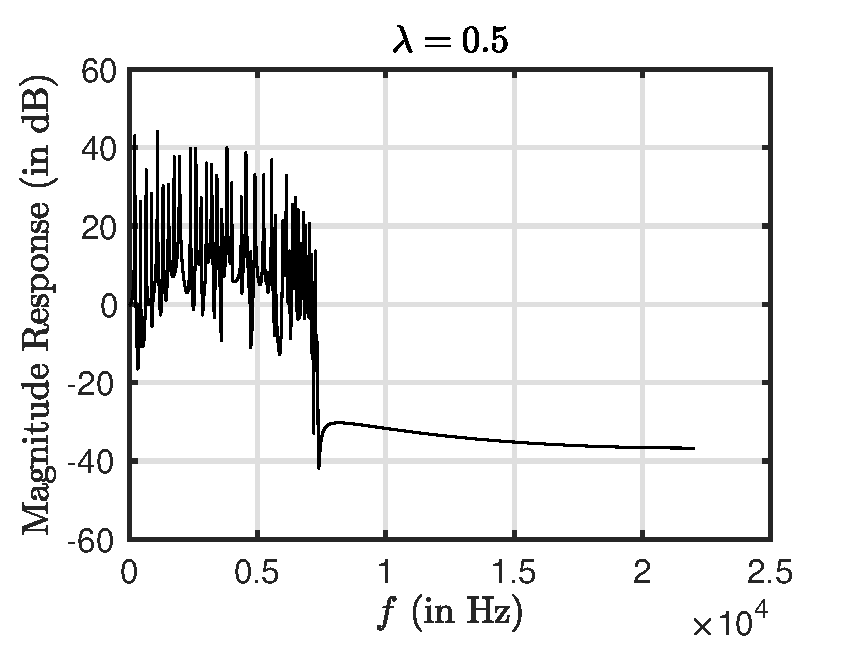
\includegraphics[width=0.3\textwidth]{Figures/bandwidthLambda05.eps}}}
    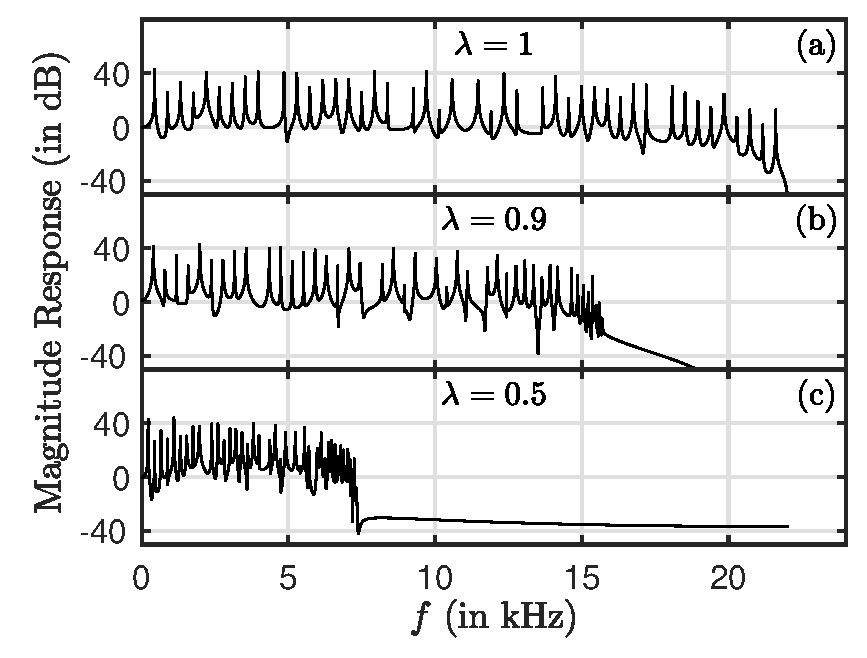
\includegraphics[width=0.9\columnwidth]{Figures/bandwidthCompact.eps}
    \caption{Bandwidths of the simulation output %at $l = 16$ 
    with $f_\text{s} = 44100$ Hz and 
    %$N = 50$ excited with a raised cosine with a width of 5 at center-location $N = 25$. The Courant number is set to 
    (a) $\lambda = 1$, (b) $\lambda = 0.9$ and (c) $\lambda = 0.5$. 
    \label{fig:bandWidths}}
\end{figure}
%
By analysing the scheme in Eq. \eqref{eq:updateEq}, it can be shown that the maximum frequency produced by the system can be calculated using \cite[Chap. 6]{bilbao2009}
\begin{equation}\label{eq:fmax}
    f_\text{max} = \frac{f_\text{s}}{\pi} \sin^{-1}(\lambda).
\end{equation}
% shown in Figure \ref{fig:bandWidthFormula}.
%
Note that only a small deviation of $\lambda$ from condition \eqref{eq:CFL} already has a profound effect on the bandwidth of the output.
%
% \begin{figure}
% %% \reprintcolumnwidth is the same in preprint and reprint for
% %% ease of use for authors:
% \includegraphics[width=0.8\reprintcolumnwidth]{bandwidthPlot}
% \caption{\label{fig:bandWidthFormula}{The effect of the Courant number $\lambda$ on the output bandwidth. \SWcomment[This figure should probably be much more compact, if not removed altogether.]}}
% \end{figure} 
Secondly, choosing $\lambda < 1$ causes numerical dispersion. See Figures \ref{fig:dispersion}b and \ref{fig:bandWidths}. Harmonic partials get closer together at higher frequencies (i.e. get more inharmonic) as $\lambda$ decreases, which is generally undesirable.

\SWcomment[can cut this paragraph $\rightarrow$] Apart from the recalculation of $\lambda$ due to the flooring operation in Eq. \eqref{eq:orderOfCalcGrid}, a reason that one would choose $\lambda < 1$ could be to decrease the total number of grid points used in the simulation by increasing $h$. This makes the simulation less computationally expensive, while keeping a desired wave speed $c$ and time step $k$. For 1-dimensional systems such as the 1D wave equation, this is rarely necessary.
